% \lipsum[4] Citing \cite{InfH} properly.
% Was ist eine \gls{guid}?
% Eine \gls{guid} kollidiert nicht gerne.

% Kabellose Technologien sind in abgelegenen Gebieten wichtig \cite{APCW2006}.
\setauthor{Martin Hausleitner}
% 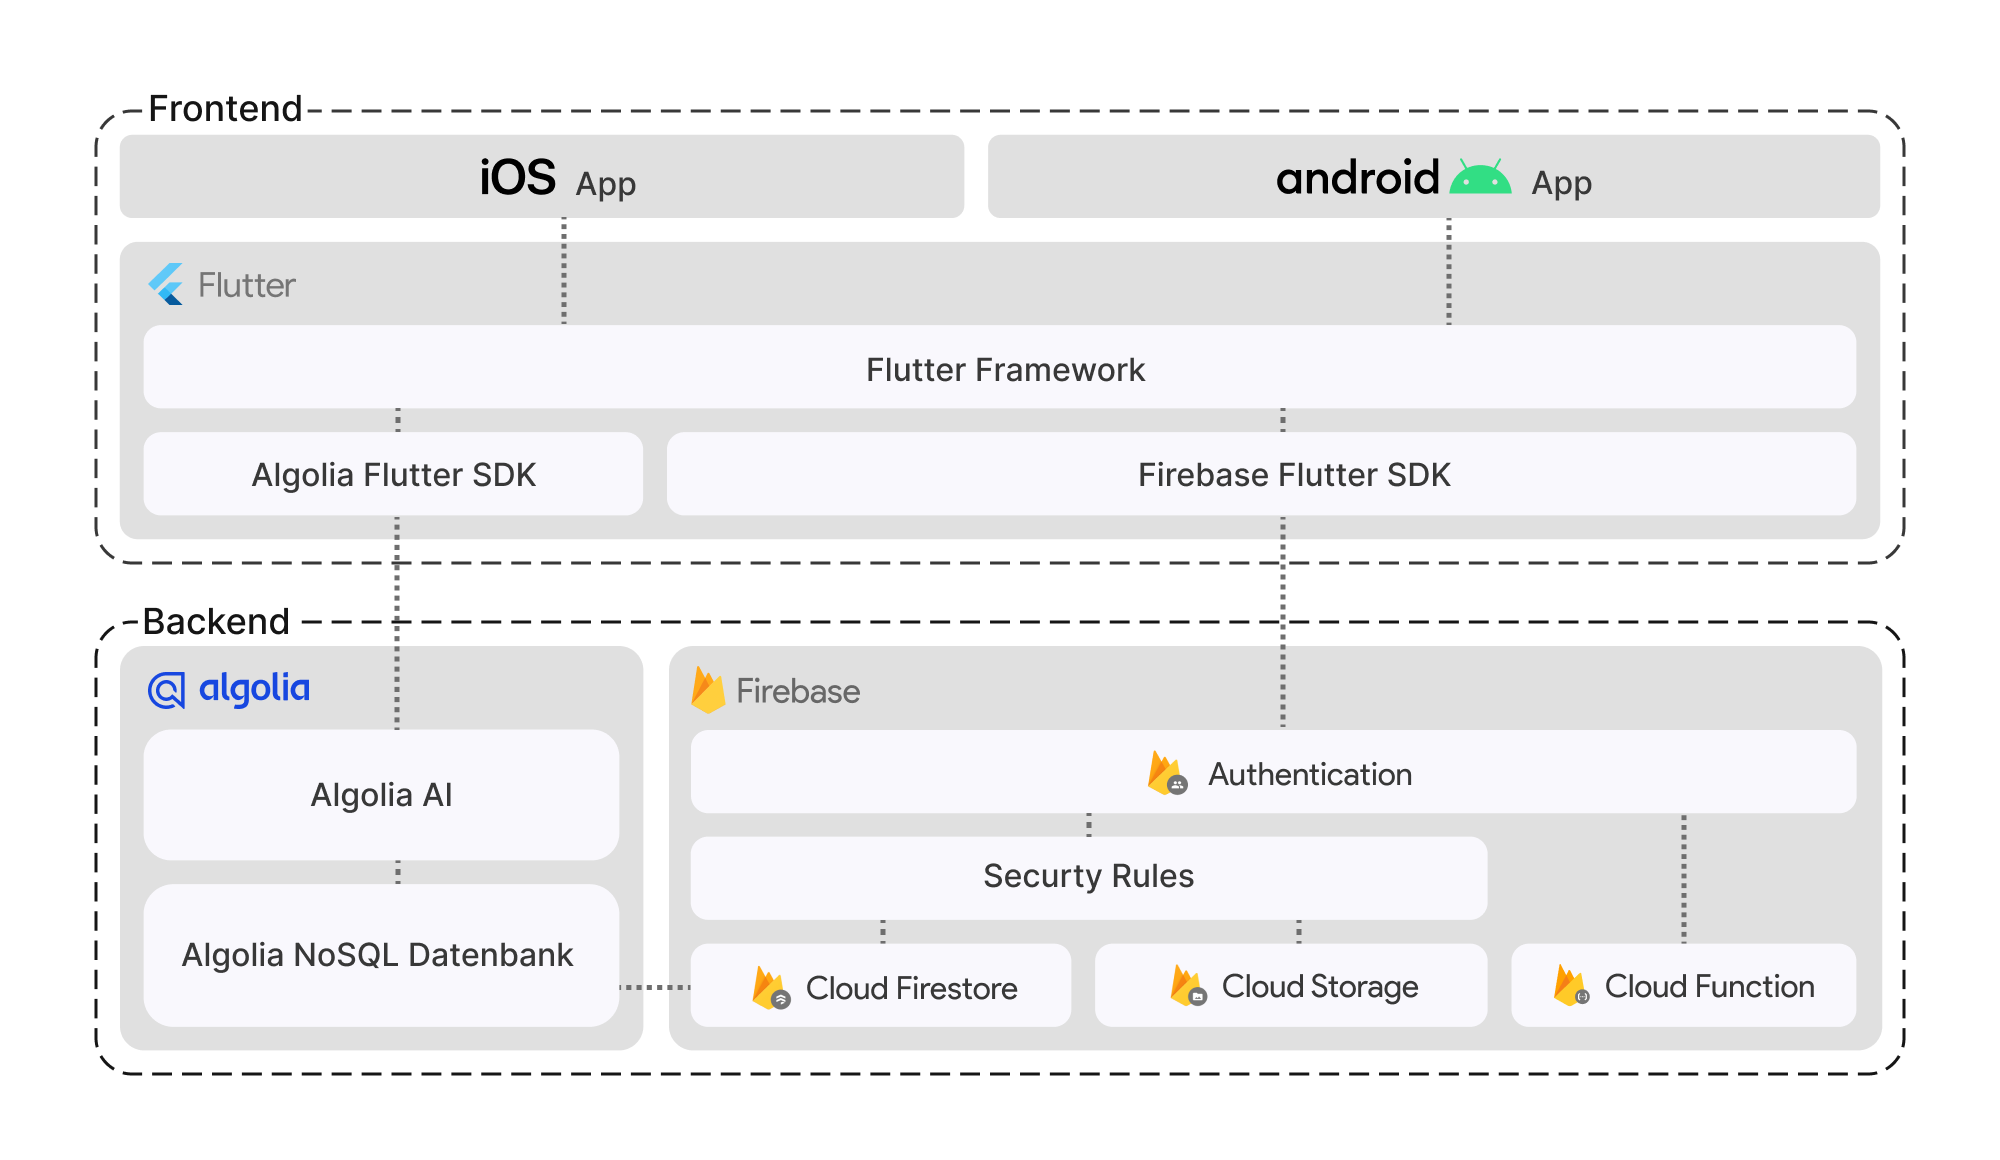
\includegraphics[width=0.2\textwidth]{pics/systemarchitektur_diagram.png}
\begin{figure}[H]
    \centering
    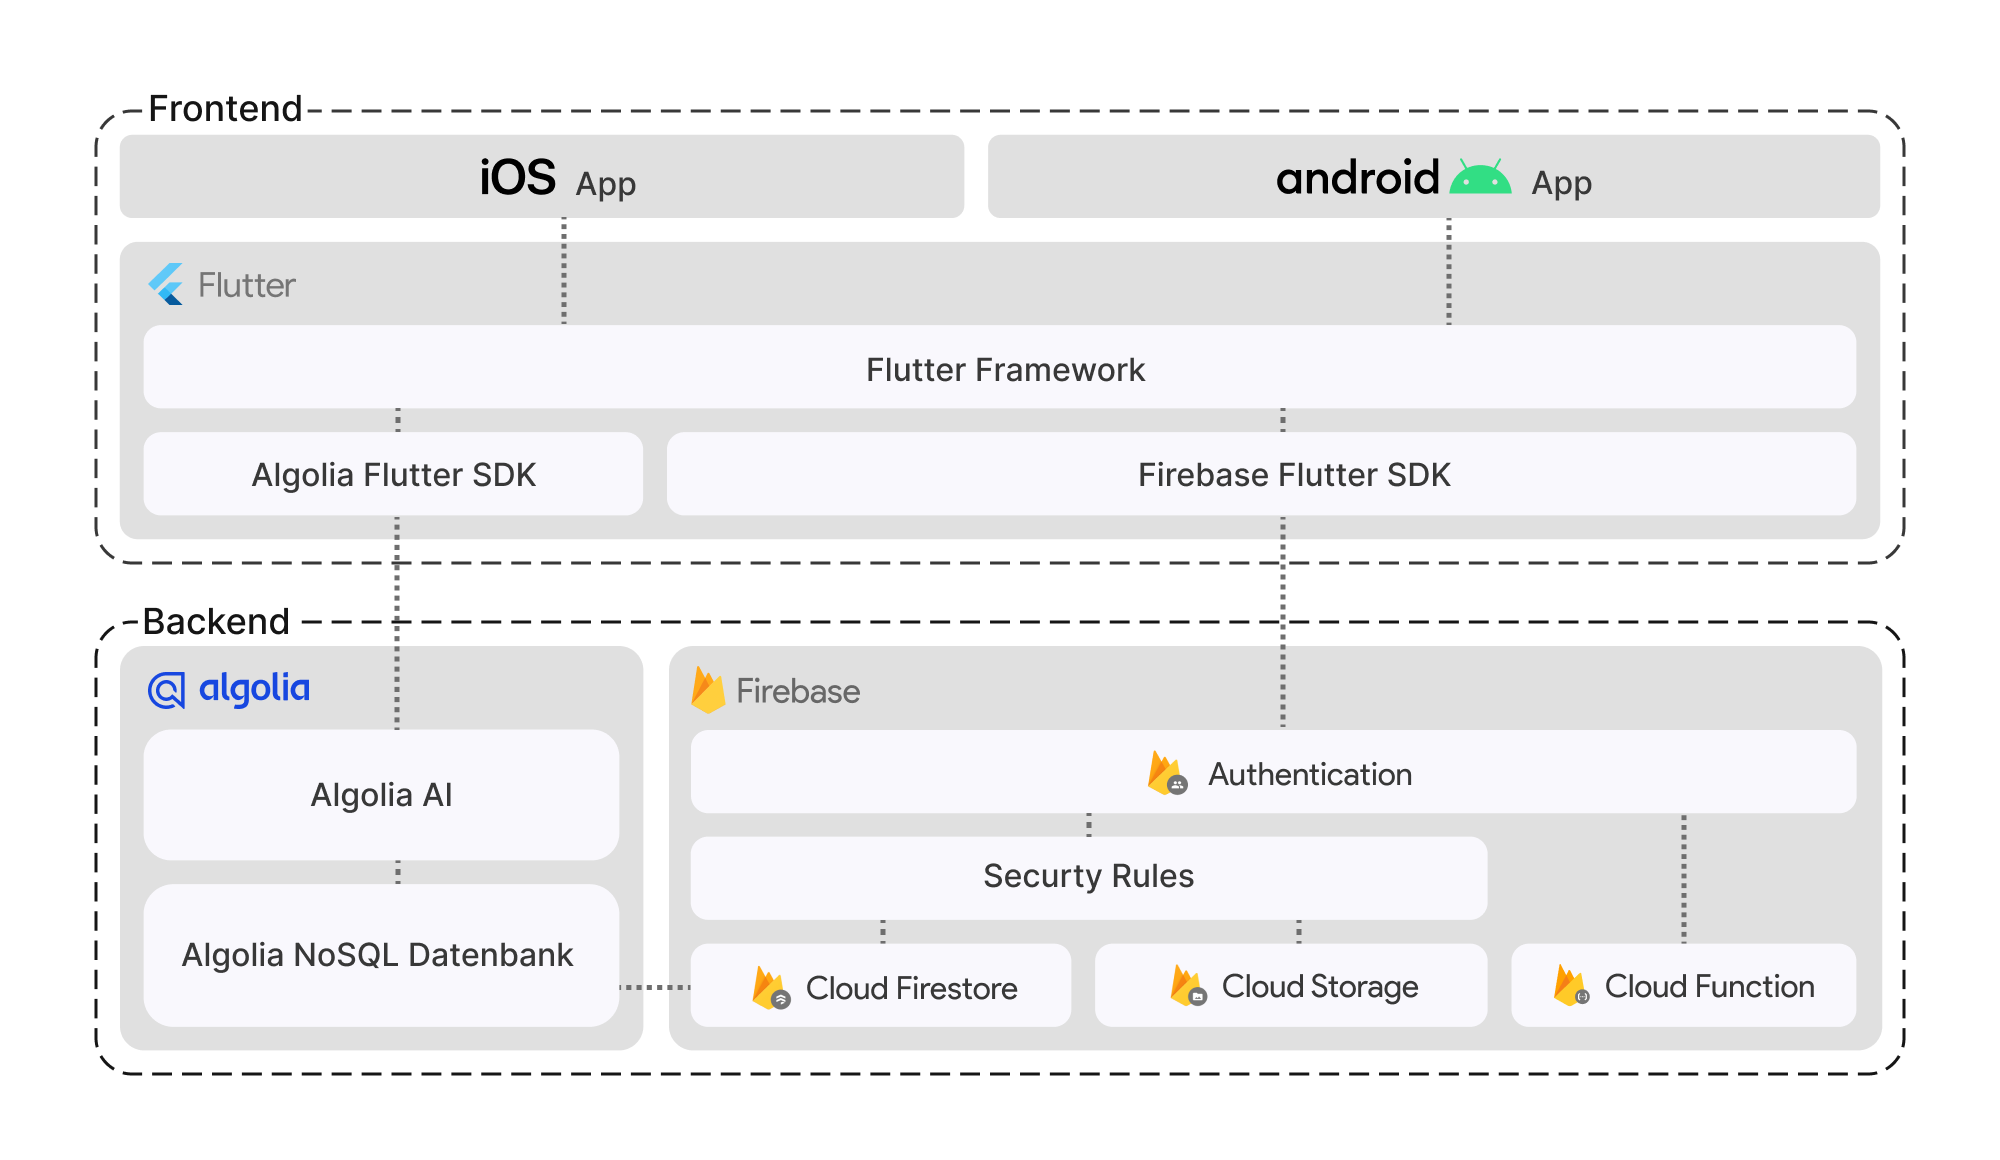
\includegraphics[width=1\textwidth]{pics/systemarchitektur_diagram.png}
    \caption{Systemarchitektur Diagramm}
    \label{fig:systemarchitektur}
\end{figure}
% todo: add systemarchitektur_diagram
% 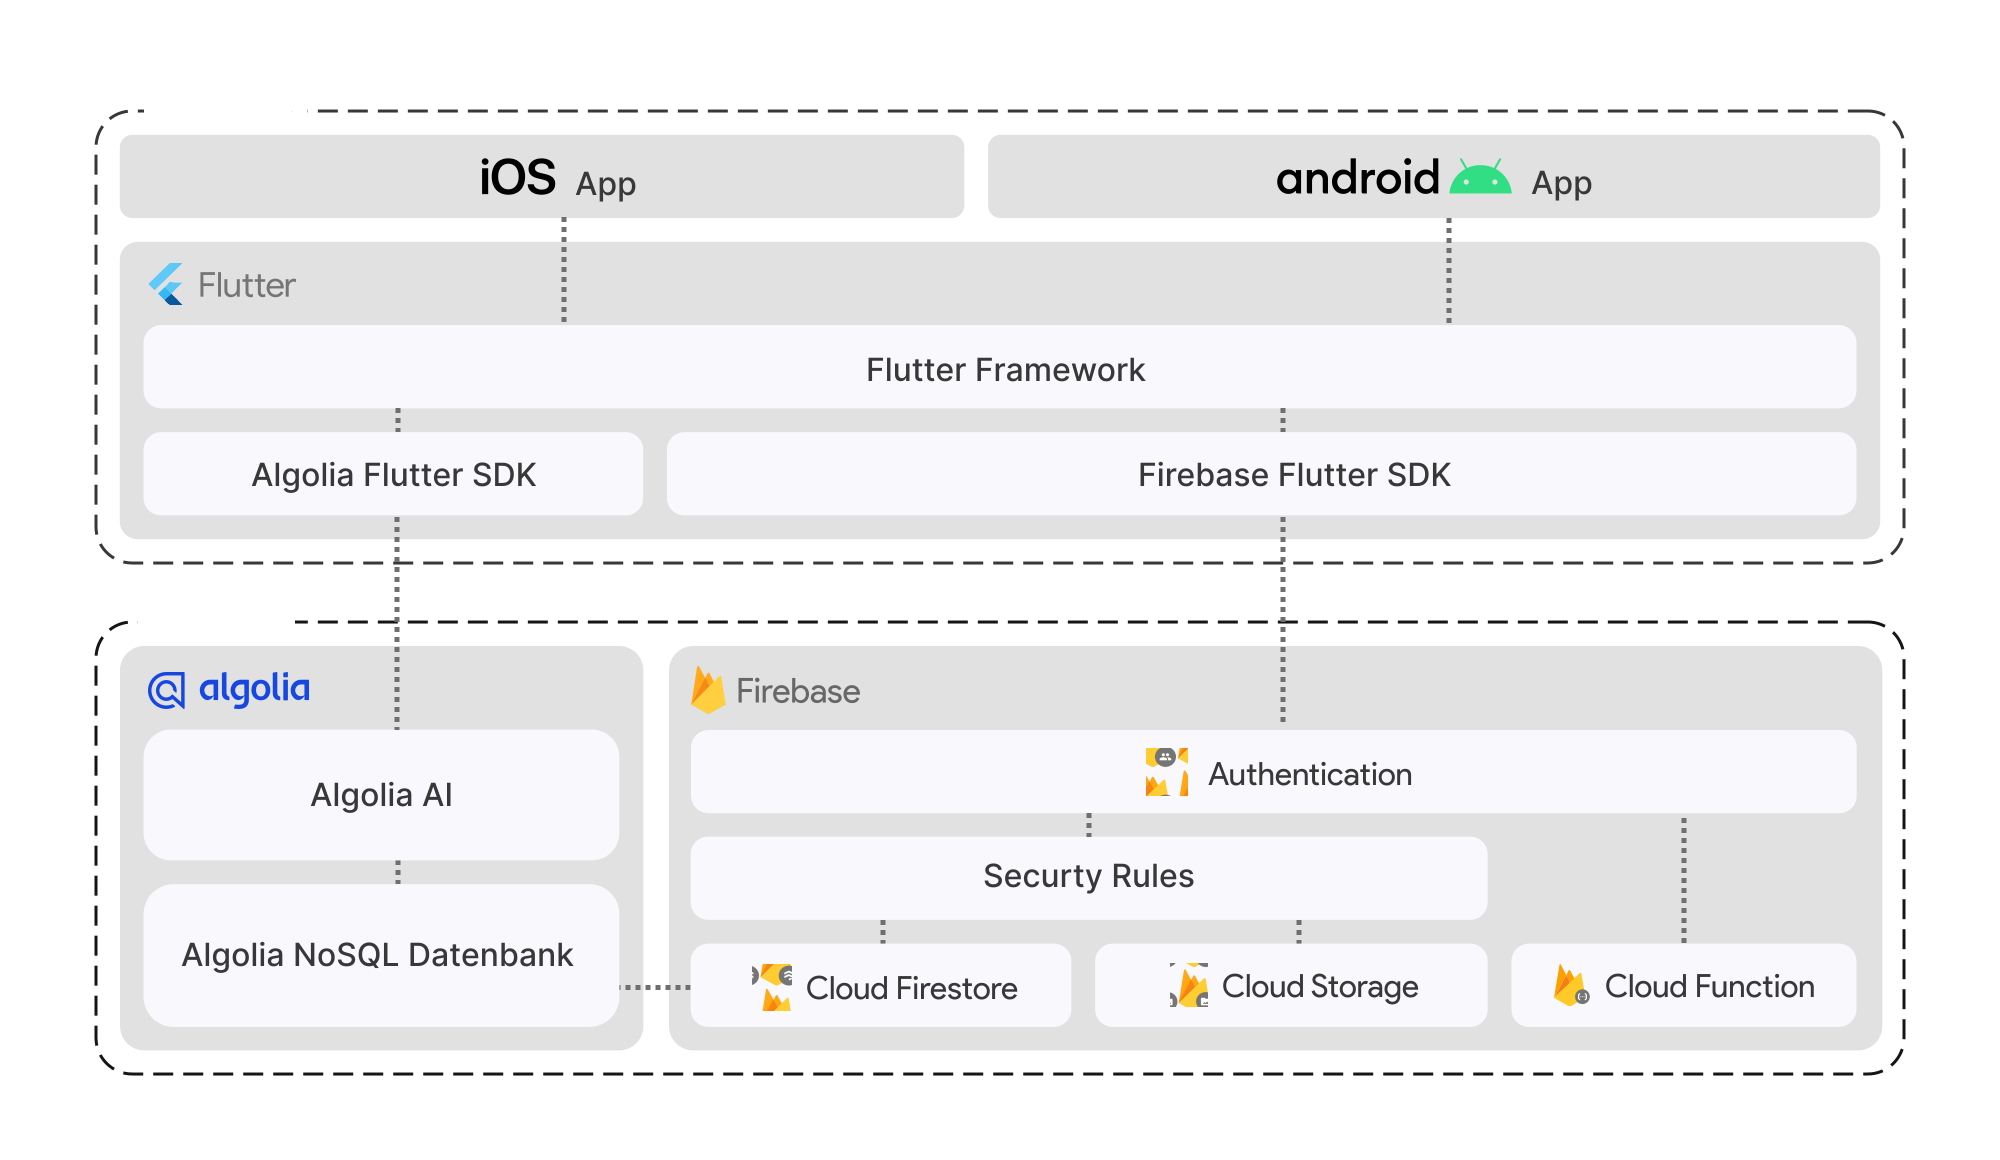
\includegraphics[width=0.2\textwidth]{pics/systemarchitektur_diagram.svg}

% \includesvg{pics/systemarchitektur_diagram.svg}
Die Abbildung \ref{fig:systemarchitektur}
veranschaulicht vereinfacht die Systemarchitektur. Der
obere Teil stellt das Frontend dar, welches vollständig im
Flutter Framework unter Verwendung der Programmiersprache
Dart entwickelt wurde. Zur Kommunikation mit dem Backend
wurden die Packages \href{https://pub.dev/packages/algolia}{Algolia
    Flutter SDK} und
\href{https://pub.dev/packages/firebase}{Firebase Flutter
    SDK} genutzt. Zur Vereinfachung wurden die Funktionen der
Firebase Flutter SDK in einem einzigen Block
zusammengefasst, während Firebase für jedes Feature ein
eigenes Package bereitstellt. Die Flutter-App wird
anschließend für iOS und Android kompiliert.

Im Backend wurde besonderer Wert auf die Implementierung von
Sicherheitsmaßnahmen gelegt. Der erste Sicherheitslayer ist
die
\href{https://firebase.google.com/docs/auth}{Firebase-Authentifizierung},
die das gesamte Authentifizierungssystem für den Zugriff auf
das Backend regelt. Firebase Cloud Functions können nur von
einem registrierten Account ausgeführt werden. Besondere
Cloud Functions verlangen darüber hinaus eine zusätzliche
Verifizierung der Adresse des Nutzers.

Die Nutzung von
\href{https://firebase.google.com/docs/firestore}{Firestore},
einer NoSQL-Datenbank von Firebase, ermöglicht die
Speicherung von Daten. Um auf die Firestore-Datenbank und
den \href{https://firebase.google.com/docs/storage}{Cloud
    Storage} zuzugreifen, ist es erforderlich, die
\href{https://firebase.google.com/docs/firestore/security/overview}{Firestore
    Security Rules} zu durchlaufen. Diese Regeln steuern
sämtliche Zugriffsrechte auf Dokumente in der Datenbank oder
dem Cloud Storage. Weiterführende Informationen dazu sind
unter dem Abschnitt \hyperref[sec:security-rules]{Security Rules} zu
finden.

Firestore verfügt nicht über eine integrierte Funktion zur
vollständigen Durchsuchung aller Dokumente, weshalb für die
Suche nach Inhalten eine externe Suchmaschine wie Algolia
erforderlich ist. Durch die Verbindung von Cloud Firestore
mit der Algolia SQL-Datenbank wird sichergestellt, dass die
Datenbanken synchronisiert werden. Ein bedeutender Vorteil
dieser Vorgehensweise, der möglicherweise zunächst als
Nachteil betrachtet werden könnte, besteht darin, dass wir
über zwei Datenbanken verfügen, die dieselben Daten
enthalten. Die Algolia-Datenbank verfügt jedoch über eine
integrierte Suchfunktion, die die Suchgeschwindigkeit und
-qualität verbessert, indem nur die Beitrag-Titel,
-Beschreibungen und -Tags gespiegelt werden, anstatt die
gesamte Datenbank zu replizieren. Weitere Informationen zu
Algolia Search ist in dem Abschnitt \ref{sec:algolia} zu finden.

\section{Flutter}
\setauthor{Sandin Habibovic}

Flutter ist ein crossplatform Frontend-Entwicklungsframework von Google, das die Entwicklung von hochperformanten, nativen Apps für iOS und Android vereinfacht. Flutter verwendet eine Widget-basierte Architektur, bei der jedes Element der Benutzeroberfläche als Widget definiert wird. Diese Architektur ermöglicht es, schnell benutzerdefinierte Benutzeroberflächen zu erstellen, die auf allen Plattformen konsistent und schnell laufen.
\\
Ein weiterer Vorteil von Flutter ist, dass es eine hohe Entwicklerproduktivität ermöglicht. Flutter bietet eine schnelle Iteration und ein Hot-Reload-Feature, das es ermöglicht, Änderungen im Code sofort zu sehen, ohne die App neu starten zu müssen. Dies ermöglicht es, schnell Fehler zu beheben und neue Funktionen hinzuzufügen.
\\
Flutter verfügt über eine umfangreiche Sammlung von Bibliotheken und Tools, die auf der offiziellen Paket-Repository-Website von Flutter, pub.dev, zu finden sind. Diese Website ist ein Verzeichnis von Paketen, dass von der Flutter-Community erstellt und gewartet wird, und bietet eine Vielzahl von Flutter-Paketen unter Open-Source-Lizenzen an. Dort können nützliche Bibliotheken gesucht und in Flutter-Projekte integriert werden. Das Vorhandensein so einer umfangreichen Sammlung von Tools und Bibliotheken ist ein wichtiger Faktor, der die Attraktivität von Flutter als Entwicklungsframework erhöht.

% Hier kommt die Beschreibung der Technologie und deren Vorteile/Nachteile, auf Basis von wissenschaftlichen Studien und Erfahrungen aus der Praxis.

Quellen:

https://docs.flutter.dev/resources/architectural-overview

https://flutter.dev/docs/resources/technical-overview,
https://pub.dev/packages/flutter


% \subsection{iOS}
% \subsubsection{CI/CD}

% \subsection{Android}
% \subsubsection{CI/CD}
% \subsubsection{Firebase App Distribution}




\section{Firebase}
\setauthor{Martin Hausleitner}
Firebase\cite{firebase} ist eine von Google entwickelte Plattform für die Entwicklung von Web- und mobilen Anwendungen. Die Plattform bietet eine Vielzahl von Tools und Diensten, die es Entwicklern ermöglichen, schnell und einfach skalierbare Anwendungen zu erstellen.

Die Systemarchitektur von Firebase basiert auf der Cloud-Computing-Technologie, bei der die Anwendungslogik und Daten in der Cloud gehostet werden. Dies bedeutet, dass Entwickler keine physischen Server oder Infrastrukturen verwalten müssen, um ihre Anwendungen zu betreiben. Stattdessen können sie sich auf die Entwicklung der Anwendungslogik konzentrieren und die Firebase-Plattform übernimmt den Rest.

Firebase bietet auch eine Echtzeit-Datenbank, die es Entwicklern ermöglicht, Daten in Echtzeit zwischen ihren Anwendungen zu synchronisieren. Darüber hinaus bietet Firebase eine Vielzahl von Tools und Diensten, darunter Authentifizierung, Benachrichtigungen, Hosting, Speicherung und vieles mehr.

Dank dieser Systemarchitektur und der bereitgestellten Tools und Dienste können Entwickler mit Firebase schnell und einfach skalierbare Anwendungen erstellen und betreiben.

\subsection{Firebase SDK}
\setauthor{Sandin Habibovic}
Firebase SDK ist eine Sammlung von Software Development Kits, die von Firebase bereitgestellt werden, um Cloud-basierte Anwendungen zu erstellen.
Firebase SDK ist für eine Vielzahl von Programmiersprachen verfügbar, darunter:
\begin{compactitem}
    \item JavaScript
    \item Swift
    \item Kotlin
    \item Java
    \item Dart von Flutter
\end{compactitem}
Die Firebase SDK bietet eine breite Palette von Funktionen, mit denen leistungsstarke Anwendungen erstellt werden können, darunter Authentifizierung, Cloud Messaging, Cloud Firestore, Realtime Database, Cloud Functions. Mit diesen Funktionen können schnell und einfach Funktionen wie Benutzerverwaltung, Datenverwaltung, Messaging und Benachrichtigungen in Anwendungen integriert werden. Außerdem gibt es zu Firebase SDK eine umfangreiche Dokumentation und Support-Tools.


\subsection{Firebase Authentication}
\author{Sandin Habibovic}

Firebase Authentication ist eine Technologie, welche die Möglichkeit bietet, Authentifizierung und Autorisierung für Apps und Webseiten unkompliziert und sicher einzubinden. Als Teil der Firebase-Plattform stellt Firebase Authentication eine vollständig gehostete Backend-Authentifizierungslösung bereit, die es erlaubt, sich auf Anwendungsentwicklung zu konzentrieren, ohne sich mit Authentifizierungs- und Sicherheitsimplementierungen auseinandersetzen zu müssen.
\\
Es stehen verschiedene Authentifizierungsoptionen zur Verfügung, wie zum Beispiel:
\begin{compactitem}
    \item E-Mail und Passwort
    \item Telefonnummer
    \item Soziale Medien wie Google, Facebook und Twitter
    \item benutzerdefinierte Authentifizierungsmethoden
\end{compactitem}

Firebase Authentication unterstützt zudem Multi-Faktor-Authentifizierung, um die Sicherheit zu verstärken und den Schutz von Benutzerkonten sicherzustellen.
\\
Die Technologie setzt auf Token-basierte Authentifizierung, um Benutzer zu erkennen und deren Authentifizierungsdaten zu verwalten. Nach erfolgreicher Authentifizierung eines Users kann die App den von Firebase Authentication bereitgestellten Token nutzen, um auf weitere Firebase-Services zuzugreifen. Dazu zählen Firestore für Datenbanken, Storage für Dateien und Functions für serverlose Berechnungen.
\\
Firebase Authentication ist auf verschiedenen Plattformen wie Web, iOS, Android und Flutter verfügbar. Die Integration in Firebase-basierte Apps ist einfach und auch die Nutzung in Verbindung mit anderen Plattformen oder Anwendungen, die nicht auf Firebase aufbauen, ist möglich.
\\
Insgesamt bietet Firebase Authentication eine sichere, skalierbare und benutzerfreundliche Lösung für die Implementierung von Authentifizierung und Autorisierung in Anwendungen und Websites.

Quellen:

https://firebase.google.com/docs/auth

https://medium.com/flutter-community/firebase-authentication-in-flutter-752d14209a8a

\subsubsection{Security Rules}\label{sec:security-rules}
\setauthor{Martin Hausleitner}
In der App ist die Sicherheit ein sehr wichtiger Faktor,
um die Vertraulichkeit und Integrität der Daten und der
Nutzer zu gewährleisten. Firebase bietet für seine
Cloud-basierten Datenbank- und Speicherlösungen - Cloud
Firestore und Cloud Storage - die sogenannten Security
Rules\cite{firebase-rules-docs}\cite{firestore-rules-firestore-nochba}\cite{storage-rules-storage-nochba}, um den Zugriff auf
die Daten und Ressourcen zu kontrollieren. Diese Regeln
definieren, wer auf welche Art und Weise auf welche Daten
zugreifen darf.

Die Security Rules für Cloud Firestore und Cloud Storage sind in einer eigenen Sprache geschrieben und werden serverseitig auf Firebase-Servern ausgeführt. Die Syntax basiert auf einer ähnlichen Struktur wie JSON und erlaubt komplexe Abfragen. Die Regeln können für eine bestimmte Sammlung oder einen bestimmten Pfad definiert werden und erlauben es, bestimmte Bedingungen für Lese- oder Schreibzugriffe zu definieren.


\begin{lstlisting}[language=Python,caption=Security Rules Beispiel]
    match /posts/{postId} {
        allow read: if request.auth.uid != null;
        allow write: if request.auth.uid == resource.data.author;
      }
\end{lstlisting}

Diese Regel definiert, dass jeder Nutzer Lesezugriff auf
alle Posts hat, aber nur der Autor des Posts ihn auch ändern
darf.

Zusammenfassend stellen die Security Rules für Cloud Firestore und Cloud Storage eine wirkungsvolle und anpassungsfähige Option dar, um Zugriffsrechte auf Daten und Ressourcen innerhalb einer Firebase-App zu kontrollieren. Mithilfe der Security Rules lässt sich gewährleisten, dass Nutzerdaten geschützt sind und ausschließlich von berechtigten Personen eingesehen oder verändert werden können.



\subsection{Cloud Firestore}
\author{Sandin Habibovic}

Cloud Firestore ist eine skalierbare, serverlose NoSQL-Datenbank, die als Teil der Firebase-Plattform angeboten wird. Diese ermöglicht es, Daten in der Cloud zu speichern, Echtzeit-Synchronisierung zwischen verschiedenen Geräten bereitzustellen und Anwendungen ohne die Notwendigkeit einer eigenen Serverinfrastruktur zu erstellen. Dadurch eignet sich Firestore besonders für mobile und Webanwendungen, die auf Skalierbarkeit, Echtzeitaktualisierungen, und hohe Verfügbarkeit angewiesen sind.
\\\\
Vorteile von Cloud Firestore:

\textbf{Skalierbarkeit:} Firestore ist in der Lage, automatisch zu skalieren, um Millionen von gleichzeitigen Verbindungen und große Mengen von Daten zu unterstützen. Das bedeutet, dass sich um Kapazitätsgrenzen keine Gedanken mehr gemacht werden muss und Anwendungen problemlos erweitert werden können, um einem wachsenden Benutzerstamm gerecht zu werden.

\textbf{Echtzeitaktualisierungen:} Firestore ermöglicht Echtzeitaktualisierungen, indem Änderungen an den Daten automatisch an alle verbundenen Geräte gepusht werden. Dies ist besonders nützlich für Anwendungen, die ständig aktualisierte Daten anzeigen oder Benutzerinteraktionen in Echtzeit verarbeiten müssen.

\textbf{Flexible Datenstrukturen:} Firestore unterstützt flexible Datenstrukturen, die es ermöglicht, Datenmodelle einfach an sich ändernde Anforderungen anzupassen. Dokumente können verschachtelte Felder, Arrays und komplexe Datenstrukturen wie Maps enthalten, was eine effiziente Organisation und Abfrage von Daten ermöglicht.

\textbf{Leistungsstarke Abfragen:} Firestore bietet leistungsstarke Abfragefunktionen, die komplexe Datenabfragen unterstützen.
Daten können sortiert, gefiltert und aggregiert werden, um genau die Informationen abrufen zu können, die benötigt werden, ohne unnötige Daten zu übertragen.

\textbf{Indexes und Abfrageoptimierung:} Um Abfragen in Firestore effizienter zu gestalten, verwendet die Datenbank automatisch erstellte Single-Field-Indexes für alle Felder in den Dokumenten. Für zusätzliche Leistung und Komplexität bei Abfragen können auch benutzerdefinierte zusammengesetzte Indexe erstellt werden, die mehrere Felder kombinieren. Diese ermöglichen es, leistungsstarke und komplexe Abfragen auszuführen, ohne die Leistung der Anwendungen zu beeinträchtigen.





Quellen:

https://firebase.google.com/docs/firestore

https://medium.com/flutter-community/firebase-cloud-firestore-in-flutter-26c6e8c6f90c



\subsubsection{Datenmodell}

Das Datenmodell in Firestore ist hierarchisch und besteht aus Dokumenten und Sammlungen, auch Collections genannt. Dokumente sind einzelne Datenobjekte, die Felder mit Werten enthalten. Sammlungen sind Container für Dokumente und können weitere Sammlungen enthalten, sogenannte Sub-Collections. Dieses hierarchische Datenmodell erlaubt es, Daten effizient zu organisieren und abzufragen.

Quellen:

https://firebase.google.com/docs/firestore/data-model

https://www.raywenderlich.com/6628345-cloud-firestore-for-flutter-getting-started

% Weitere wichtige punkte:

% \begin{compactitem}
%     \item Präsentation des eigenen Datenmodells in der Arbeit.
%     \item Diagramme werden verwendet, um das Modell zu präsentieren und Entscheidungen zu erläutern und zu begründen.
%     \item Anforderungen der App-Architektur werden dabei berücksichtigt werden.
%     \item Performance, Skalierbarkeit und Strukturierung können thematisiert werden.
%     \item Zur Veranschaulichung unserer eigenen Datenmodell-Entwicklung kann auf ein Beispiel-Datenmodell-Diagramm auf der offiziellen Firebase-Website verwiesen werden, welches uns als Orientierungshilfe diente.
% \end{compactitem}

% Beispiel-Datenmodell-Diagramm Quelle:

% https://firebase.google.com/docs/firestore/data-model\#structure\_your\_data

\subsection{Cloud Storage}

Cloud Storage ist eine Technologie von Firebase, die es ermöglicht, Dateien wie Dokumente, Videos und besonders Bilder, wie Profilbilder, sicher und effizient in der Cloud zu speichern und abzurufen.
\\
Firebase Cloud Storage ist ein leistungsstarkes, sicheres und skalierbares Speichersystem, das auf Google Cloud Storage aufbaut und speziell für die Anforderungen mobiler und Webanwendungen entwickelt wurde. Es ermöglicht, Dateien direkt von den Geräten der User in die Cloud hochzuladen, ohne dass ein eigener Server erforderlich ist. Cloud Storage bietet zudem Funktionen wie Sicherheitsregeln, die den Zugriff auf Dateien auf Benutzerbasis steuern, sowie On-the-fly-Komprimierung und Caching, um die Netzwerkbandbreite zu optimieren und die Leistung zu verbessern.
\\
Die Integration von Cloud Storage in die App ist einfach und effizient. Durch die von Firebase bereitgestellten SDKs wird der nahtlose Zugriff auf Cloud Storage und Dateioperationen wie Hochladen, Herunterladen, Anzeigen und Löschen ermöglicht.
\\
Ein wesentlicher Aspekt von Cloud Storage ist die Sicherheit und Zugriffskontrolle. Firebase Cloud Storage ermöglicht, granulare Sicherheitsregeln zu definieren, die den Zugriff auf Dateien basierend auf verschiedenen Kriterien wie Benutzer-Authentifizierung, Dateipfade und Metadaten steuern. Die Sicherheitsregeln sind in einer einfachen, aber leistungsfähigen Sprache geschrieben und können flexibel an die Anforderungen der App angepasst werden. Durch die Kombination von Cloud Storage-Sicherheitsregeln mit Firebase Authentication kann sichergestellt werden, dass nur berechtigte User auf die entsprechenden Dateien zugreifen und Operationen ausführen können.
\\
Firebase Cloud Storage ist auf Performance und Skalierbarkeit ausgelegt und eignet sich sowohl für kleine als auch für große Anwendungen mit hohem Datenaufkommen. Durch die Verwendung von Google Cloud Storage als Basis profitiert Cloud Storage von der globalen Infrastruktur und den Optimierungen von Google, um eine hohe Verfügbarkeit, geringe Latenz und hohe Übertragungsgeschwindigkeiten zu gewährleisten. Zudem können Funktionen wie automatische Komprimierung und Caching genutzt werden, um die Netzwerkbandbreite zu optimieren und die Ladezeiten für die User zu minimieren. Da Firebase Cloud Storage automatisch skaliert, können Anwendungen bei steigenden Nutzerzahlen und Datenvolumen sicher und reibungslos funktionieren.

Quellen:

https://firebase.google.com/docs/storage

https://medium.com/flutter-community/firebase-cloud-storage-in-flutter-flutter-an-firebase-tutorial-c5de7835c6cd

\subsection{Firebase Cloud Functions}
\setauthor{Martin Hausleitner}
Dank Firebase Cloud Functions\cite{firebase-cloud-functions} lässt sich Business-Logik, wie etwa der Registrierungsprozess und viele andere logische Vorgänge, einfach und effektiv in der Cloud umsetzen. Die Entscheidung, die Funktionen in TypeScript zu verfassen, ergibt sich aus zahlreichen Vorteilen, wie statischer Typisierung, verbesserter IDE-Unterstützung und erhöhter Code-Lesbarkeit.

Der Registrierungsprozess verdeutlicht den Einsatz von Firebase Cloud Functions. Statt einer monolithischen Anwendung, welche alles auf einem Server verwaltet, wird die Logik in kleinere Funktionen zerlegt, die jeweils spezifische Aufgaben erfüllen.

Firebase Cloud Functions bieten viele Vorzüge, darunter einfache Skalierbarkeit und automatische Verteilung zur Bewältigung hoher Lasten. Die Funktionen lassen sich zudem einfach testen und debuggen, indem lokale Emulatoren genutzt werden, bevor sie in der Cloud bereitgestellt werden.

Insgesamt stellen Firebase Cloud Functions eine ausgezeichnete Möglichkeit dar, Business-Logik in der Cloud abzubilden und Anwendungen zu skalieren und zu optimieren. Durch den Einsatz von TypeScript bleibt der Code sauber, robust und wartungsfreundlich.

\section{Algolia Search}\label{sec:algolia}
\setauthor{Arsham Edalatkhah}

Algolia ist eine Suchtechnologie, die es Entwicklern ermöglicht, relevante und schnelle Suchergebnisse für ihre Anwendungen bereitzustellen. Diese Technologie wurde speziell für moderne Anforderungen im Bereich der Suche entwickelt und bietet Funktionen wie automatisches Vervollständigen, Sortierung nach Relevanz und Suche nach Kategorien.

Im Zuge der Nochba-App hat sich das Team für die Verwendung der Algolia-Suche in Verbindung mit einem Firebase-Backend entschieden. Aus der Perspektive der Systemarchitektur umfasst dieses Konzept zwei wesentliche Teile: die Firebase-Datenbank zur Speicherung und Verwaltung von Daten und den 'Algolia'-Suchdienst zur Bereitstellung schneller und effizienter Suchfunktionalität.

Die in der Firebase-Datenbank gespeicherten Daten werden mit Algolia synchronisiert, um sicherzustellen, dass die Suchergebnisse aktuell und genau sind. Diese Kombination von Technologien ermöglicht es dem Team, die Echtzeit-Fähigkeiten und die einfache Skalierbarkeit von Firebase zu nutzen und gleichzeitig von den hoch entwickelten Suchfunktionen von Algolia zu profitieren.

Hinsichtlich der Preisgestaltung bietet Algolia eine kostenlose Stufe an, die 10.000 Suchvorgänge und 10.000 Indexierungsvorgänge pro Monat umfasst. Dieses kostenlose Angebot eignet sich für die Testphase der Nochba-App, weil man damit genügend Such- und Indexierungsoperationen durchführen kann, um die Suche und die Leistung zu analysieren. Wenn die App größer wird und die Anzahl der Nutzer steigt, kann das Team ein Upgrade auf einen kostenpflichtigen Plan in Betracht ziehen, um den höheren Ansprüchen nachzukommen.

Die Integration von Algolia in eine App-Architektur ist einfach durchzuführen und benötigt keine langen Zeiträume. Es stellt eine RESTful API zur Verfügung, die direkt von der Anwendung aufgerufen werden kann. Es gibt auch integrierte Lösungen für verschiedene Backend-Systeme wie Firebase, was die Integration noch einfacher macht.

Durch die Verwendung von Algolia kann eine Anwendung schnelle und relevante Suchergebnisse bereitstellen, was das Nutzererlebnis verbessert. Es gibt auch eine Vielzahl von Tools und Funktionen, die Entwicklern bei der Optimierung ihrer Suchergebnisse helfen, um die besten Ergebnisse für ihre Nutzer zu erzielen.

\subsubsection{Firebase Cloud Function}

Beschreibung der Firebase Cloud Functions und deren Rolle in der Algolia Integration.

Quellen:

https://firebase.google.com/docs/functions

https://www.algolia.com/doc/guides/sending-and-managing-data/send-and-update-your-data/tutorials/firebase-algolia/
